% Created by Jim Finnis
% Date Wed Feb 24 13:48:57 2021


\section{The data model}
The data model consists of two parts --- the data itself (largely
image cube data) and the graph. By far the most important kind of data
from the point of view of this document is the image data, which ties
into the user interface in complex ways. Other forms of data do exist,
but these are much simpler.

\subsection{ImageCube}
Most classes making up the image data 
model are described in the \texttt{pancamimage.py} file, including the main \texttt{ImageCube}
class. Some additional classes describing where images can come from are in \texttt{channelsource.py}.
The model is shown in outline in Fig.~\ref{image.png} although some links to channel sources
and mapping from nodes are omitted; these will be explained later.

\begin{figure}[ht]
\center
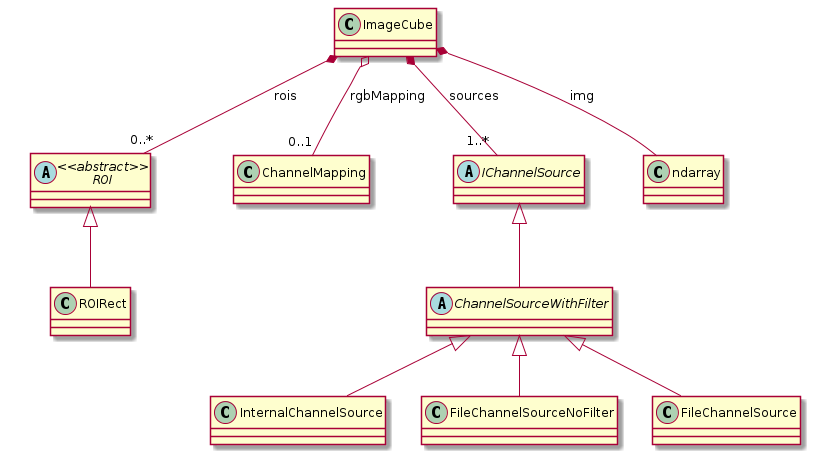
\includegraphics[width=5in]{image.png}
\caption{Outline UML class diagram of image model}
\label{image.png}
\end{figure}
